%
% examples.tex
%
% (c) 2019 Prof Dr Andreas Mueller
%
\chapter{Introductory examples of partial differential equations
\label{chapter:examples}}
\lhead{Introductory examples}
In this chapter we present a few partial differential equations
of prime practical importance which will also serve us as case
studies to illustrate general theorems and solution techniques.
The examples illustrate
\begin{enumerate}
\item
the manifold applications of the theory of partial differential equations,
\item
three completely different types of partial differential equations
that lead to wastly different solution algorithms and
\item
the importance of the boundary and initial conditions, or more generally
of the domain of the problem.
\end{enumerate}

%
% waveequation.tex -- the wave equation
%
% (c) 2019 Prof Dr Andreas Mueller
%
\rhead{Wave equation}
\section{Wave equation\label{beispiele:wellengleichung}}
\index{wave equation}
In the simplest form, this equation describes the motion
of a string of a guitar or a piano, or the air column of a 
wind instrument.
It can be generalized to vibration of a membrane or the fluid inside
an arbitrary threedimensional volume.
Electromagnetic waves can be modelled with this equation just as
well as the waves on the surface of a lake.

\subsection{The differential equation of a vibrating string}
\index{string}
Let a thin string with linear mass density $\mu$ be mounted between
the points $x=0$ and $x=l$ (figure~\ref{saite}).
The force $F$ at the end points of the string maintains its tension.
We ask for a partial differential that describes the motion of a
string after we bring it into a certain shape and let it go at time $t=0$.

The state of the string at any time can be described by a function
$u(x,t)$, which measures the deflection of the string from the straight
line between the two end points.
We need to find a differential equation for the function $u$.

From this problem description we can already derive some information
about the solution.
We note that the end points of the string are fixed, so
\[
u(0,t)=u(l,t)=0\quad\forall t\ge 0.
\]
We call this a boundary condition.
At time $t=0$ the string is supposed to have a given shape.
This is the situation of the guitar player who plucks a string and then
lets it go.
Mathematically we can formulate this as the initial condition
\[
u(x,0) = f(x)\qquad 0 < x < l.
\]
A piano however works differently, at $t=0$ it imparts a certain velocity
profile on the string, or in mathematical form
\[
\frac{\partial}{\partial t}u(0,x) = g(x),\qquad 0<x<l.
\]

\begin{figure}
\begin{center}
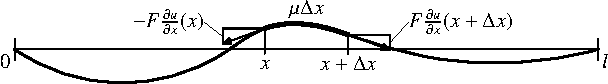
\includegraphics[width=\hsize]{../common/images/saite-1}
\end{center}
\caption{Derivation of the differential equation of a vibrating string
\label{saite}}
\end{figure}
To derive the equation of motion of a vibrating string, we consider
a small section of the string between coordinates $x$ and $x+\Delta x$
(figure \ref{saite}).
Newton's law says that the acceleration of this piece of string 
is proportional to forces acting on it, with the mass as proportionality
factor.
The mass of this piece of the string is $m=\mu\Delta x$.
At each end of the segment, a force of absolute value $F$ pulls the piece
outward, but these forces don't necessarily have the same direction,
resulting in a vertical force component.
This component turns out to be
\[
F\frac{\partial u}{\partial x}(x+\Delta x)-F\frac{\partial u}{\partial x}(x).
\]
Since the acceleration of the string segment is
$\displaystyle\frac{\partial^2u}{\partial t^2}$
we obtain the equation of motion
\begin{align*}
\mu\Delta x\frac{\partial^2u}{\partial t^2}(x)&=
F\frac{\partial u}{\partial x}(x+\Delta x)-F\frac{\partial u}{\partial x}(x)\\
\Rightarrow\qquad
\frac{\mu}{F}\frac{\partial^2u}{\partial t^2}(x)&=
\frac1{\Delta x}\left(\frac{\partial u}{\partial x}(x+\Delta x)-\frac{\partial u}{\partial x}(x)\right)
\end{align*}
By going to the limit 
$\Delta x\to 0$ we obtain the partial differential equation
\begin{equation}
\frac{\partial^2u}{\partial t^2}=\frac{F}{\mu}\frac{\partial^2u}{\partial x^2}.
\label{examples:wave-equation}
\end{equation}
This is the wave equation.
The coefficient
$\frac{F}{\mu}$
in \eqref{examples:wave-equation}
has the dimension of a velocity squared, it is the velocity by which waves
propagate along the string.

\subsection{The differential equation of an organ pipe}
\index{organ pipe}
The analysis of the vibrating string carries over almost unchanged
to a pipe organ (or any other wind instrument).
The deflection of the string is replaced by a deviation of the pressure.
We then obtain the wave equation
\[
\frac{\partial^2p}{\partial t^2}=
a^2\frac{\partial^2p}{\partial x^2}
\]
Again, $a$ is the velocity by which pressure changes propagate in
the medium, i.~e.~the speed of sound.

The boundary conditions, however, turn out to be more complicated and more
interesting.
If the end of the pipe is closed, then the air cannot move at this end.
Because movement of the air in the pipe is always associated with pressure
differences, we conclude that there cannot be a pressure gradient at the
end of the pipe in this case.
This leads to the so called {\em Neumann boundary condition}
\index{Neumann boundary conditions}
\[
\frac{\partial}{\partial x}p(x_0,t) = 0\qquad \text{for $t>0.$}
\]

On the other hand, if the pipe is open, then there is nothing that keeps
the air in the pipe, air can move freely, and the pressure is always equal
to that the surrounding air.
This leads to the so called {\em Dirichlet boundary condition}
\index{Dirichlet boundary conditions}
\[
u(x_0,t)=0\qquad \text{for $t>0.$}
\]

\subsection{Wave equation in two and three dimensions}
In analogy with the differential equation of a string we can derive the
equation of motion of a membrane fixed around its perimeter.
\index{membrane}
Let $G$ be a two-dimensional domain\footnote{The precise definition of
the term {\em domain} will be given later.}
in $\mathbb R^2$ describing the shape
of the membrane, and let $\gamma=\partial G\subset G$ be
the boundary curve of the domain.
Then the deviation of the membrane from zero position is a function
\[
 u \colon G\times \mathbb R_{t \ge 0}\to\mathbb R\colon (x,y,t)\mapsto  u (x,y,t)
\]
The membrane is fixed at the boundary, so $u$ has to satisfy the
boundary conditions
\[
 u (x,y,t)=0\qquad \forall (x,y)\in\partial G,\quad t\ge 0.
\]
The function satisfies the partial differential equation
\[
\frac{\partial^2 u }{\partial t^2}
=
c^2\left(\frac{\partial^2 u }{\partial x^2}
+
\frac{\partial^2 u }{\partial y^2}\right)
\qquad\text{in $G$.}
\]
The solution is only determined if we know the initial shape of the
membrane and its velocity. 
This leads to the initial conditions
\begin{equation}
\left.
\begin{aligned}
 u (x,y,0)&=f(x,y)
\frac{\partial}{\partial t} u(x,y,0)=g(x,y)
\end{aligned}
\right\}\qquad
\forall (x,y)\in G.
\end{equation}

In three dimensions, the wave equation becomes
\[
\frac{\partial^2 u }{\partial t^2}
=c^2\left(\frac{\partial^2 u }{\partial x^2}
+\frac{\partial^2 u }{\partial y^2}
+\frac{\partial^2 u }{\partial z^2}
\right).
\]
The additional data required also becomes a bit more involved.
First we have to define a domain 
$G\subset \mathbb R^3$ in threedimensional space.
The boundary of this volume must be a sufficiently smooth surface.
The solution then has to satisfy the boundary conditions
$u(x,y,z,t) = 0$ for points
$(x,y,z)\in \partial G$ on the boundary surface of $G$.

\subsection{The Laplace operator\label{beispiele:laplaceoperator}}
\index{Laplace operator}
\index{laplacian}
In all the problems discussed so far, the Laplace operator,
also called laplacian,
\[
\Delta
=
\begin{cases}
\displaystyle
\frac{\partial^2}{\partial x^2}
+\frac{\partial^2}{\partial y^2}&\qquad\text{two dimensions}\\
\\
\displaystyle
\frac{\partial^2}{\partial x^2}
+\frac{\partial^2}{\partial y^2}
+\frac{\partial^2}{\partial z^2}&\qquad\text{three dimensions}
\end{cases}
\]
appeared.
In fact, up to a constant factor, it turns out that this is the only
linear operator involving only second derivatives that is invariant
with respect to arbitrary rotations of the coordinate system.
This means that for a problem that is rotationally symmetrc, this is
the only operator that can have a physical meaning independent
of the choice of coordinate system.


%
% poissonproblem.tex
%
% (c) 2019 Prof Dr Andreas Mueller
%
\section{Poisson problem}
\rhead{Poisson problem}
\label{poisson-problem}
This section describes two examples of elliptic partial differential
equations, to be expanded on in chapter~\ref{chapter-elliptisch}.

\subsection{Minimal surfaces\label{beispiele:minimal surfaces}}
What shape will a soap film take when it is lifted to height
$f(x,y)$ at the boundary $(x,y)\in\gamma$ of 
a two dimensional domain $G\subset \mathbb R^2$?
If we describe the height of the soap film using a function
$u(x,y)$, we expect to find a partial differential equation for $u$
with boundary condition $f$.
\index{minimal surface}

In the derivation of the equation of motion for the vibrating string
we learned that the force accelerating the string depended on the
curvature of the string.
For the soap film, the restoring force is provided by the surface
tension which is equally strong in each direction of the film.
The soap film has two directions in which it can curve, roughly
given by the second partial derivatives $\partial^2 u/\partial x^2$ and
$\partial^2 u/\partial y^2$.
We therefore expect that force accelerating the film proportional
to the sum of these second derivatives with respect to $x$ and $y$.
Since the film is supposed not to move, we expect the differential
equation:
\[
\frac{\partial^2 u }{\partial x^2}+\frac{\partial^2 u }{\partial y^2}
=\Delta u =0.
\]

This simplified derivation is only valid for small deviations.
More generally, the so called mean curvature of the surface needs
to vanish for a minimal surface.
\index{mean curvature}

\subsection{Electric potential}
\index{electric potential}
In electrodynamics it is shown that a static electric field is a 
gradient field, i.~e.~there is a potential $\varphi$ such that the
electric field
\[
\vec E=\operatorname{grad}\varphi
\]
is its gradient.
It is also shown that the sources of the field are the electric charges.
Without charges, there are no sources to the field.
The mathematical expression of these facts is that 
the electric field satisfies the same partial differential equation
\[
\operatorname{div}\vec E=\operatorname{div}\operatorname{grad}\varphi
=\Delta \varphi=0
\]
as a minimal surface.
This problem seems to have mathematical significance independent of the
particular application.


%
% heatequation.tex -- heat equation
%
% (c) 2008 Prof Dr Andreas Mueller
%
\rhead{Heat equation}
\section{Heat equation}
The heat equation is a prototype for a so called parabolic differential
equation.
Such equations are also used to describe diffusion processes.
The Schrödinger equation, the basis of quantum mechanics, is also of this type.

We derive the heat equation for the one dimensional case.
We examine a rod of length $l$ between $x$-coordinates $0$ and $l$
and strive to compute the temperature distribution $T(x,t)$ for 
$0<x<l$ and for all times $t>0$.
We need the initial temperature distribution, which we call
$T(x,0) = f(x)$.
We expect to solve this problem using a partial differential equation.

The heat that flows in a time interval $\Delta t$ through the rod at
coordinate $x$ is proportional to the temperature gradient at that point.
The amount of heat flowing into the section  of the rod between
$x$ and $x+\Delta x$ is therefore proprtional to
\[
\frac{\partial T}{\partial x}(x+\Delta x)-\frac{\partial T}{\partial x}(x).
\]
This additional heat lets the temperature if the segment rise, depending
on the heat capacity of the material.
The volume of the segment is $\Delta x$, the temperature change is smaller
when the volume is larger.
It becomes
\[
\Delta T
=
\kappa
\frac{1}{\Delta x}
\biggl(
\frac{\partial T}{\partial x}(x+\Delta x)-\frac{\partial T}{\partial x}(x).
\biggr) \Delta t.
\]
Dividing by $\Delta t$ and going to the limits $\Delta t\to 0$
and $\Delta x\to 0$ leads to
\[
\lim_{\Delta t\to 0}\frac{\Delta T}{\Delta t}
=
\frac{\partial T}{\partial t}
=
\kappa
\lim_{\Delta x\to 0}\frac1{\Delta x}\left(\frac{\partial T}{\partial x}(x+\Delta x)-\frac{\partial T}{\partial x}(x)\right)
=\kappa\frac{\partial^2T}{\partial x^2}.
\]

Again we have to specify suitable initial and boundary conditions.
As initial condition we already have found
\[
T(x,0)=f(x)\qquad \forall x\in[0,l].
\]
As a boundary condition at the end of the rod we could prescribe the
temperature.
In physics terms this means that both ends of the rod are in contact
with a heat reservoir at constant temperature.
If we prescribe the derivatives of $T$ with respect to $x$ at $x=0$ and
$x=l$, we fix the flow of heat into the rod.
In particular, requiring
\[
\frac{\partial T}{\partial x} = 0
\]
means that no heat flows through the ends of the rod, the rod is
thermally isolated from its environment.


%
% supersonic.tex -- the equation for a supersonic flow
%
% (c) 2008 Prof Dr Andreas Mueller
%
\rhead{Supersonic flow}
\section{Supersonic flow}
In the year 1928, Jakob Ackeret habilitated at ETH Zürich with a 
\index{Ackeret, Jakob}
\index{supersonic flow}
paper with the title
``Über Luft-Kräfte bei sehr grossen
Geschwindigkeiten insbesondere bei ebenen Strömungen''.
He showed how to compute the aerodynamic forces on an object
in a supersonic flow using a linear approximation.
The velocity field of the gas that enters the region of interest with
velocity $v_1$ in $x$-direction turns out to be the gradient of
a function $\varphi(x,y,z)$ that satisfies the equation
\[
(1-\textit{Ma}_1)\frac{\partial^2\varphi}{\partial x^2}
+
\frac{\partial^2\varphi}{\partial y^2}
+
\frac{\partial^2\varphi}{\partial z^2}=0.
\]
The expression
$\textit{Ma}_1=\frac{v_1}{c_1}$ is called the Mach number of the flow,
$c_1$ is the speed of sound.
The Mach number expresses the flow velocity in units of the speed of sound.

For small velocities, we have $(1-\textit{Ma}_1)>0$, and the equation
becomes similar to the Poisson problem.
This is called potential flow.

For supersonic flow, however, the first term
$(1-\textit{Ma}_1) < 0$
changes sign, and the equation behaves like a wave equation.
In fact, the flow shows shock waves propagating away from the object
and thus carrying away its energy
(figure~\ref{ueberschall2d}).
By carefully analyzing this solution, Ackeret was able to compute
aerodynamic drag due to these shock waves.
\index{areodynamic drag}
\index{shock waves}


%
% beamequation.tex -- beam equation
%
% (c) 2019 Prof Dr Andreas Mueller
%
\rhead{Beam equation}
\section{Beam equation}
In the derivation of the differential equation of a string we
have used that fact that the string does not resist to being
bent.
Even large curvature of the string does not result in force trying
to straighten it out again.
A beam behaves completely differently.
Bending the beam creates internal stresses in the beam that
try to bring the beam back to its original shape.
We don't try to explain these forces, but it is natural to expect that
they will be proportional to the curvature and thus to the second
derivatives of the beam.
In addition, the are proportional to some material constants
(the elastic modulus $E$)
and to a property derived from the cross section of the beam,
namely the second moment $I$%
\footnote{The definition of $I$ is not relevant for the present
discussion.}.

A segment of length $\Delta x$ of a beam with linear mass density $m$
therefore experiences the following force components:
\begin{enumerate}
\item
Restoring forces caused by the stresses in the beam:
$-EI\frac{\partial^4}{\partial^4 x}w(t,x)\Delta x$
\item
Damping
$-b\frac{\partial}{\partial t}w(t,x)\Delta x$
\item
Exterior forces, e.~g.~loads on the beam:
$q(x,t)\Delta x$
\end{enumerate}
By Newton's law, these forces musst sum up to
\[
m\Delta x\frac{\partial^2}{\partial^2 t}w(t,x).
\]
By going to the limit $\Delta x\to 0$ once more we get
\begin{align*}
m\frac{\partial^2}{\partial^2t}w(t,x)
&=-EI\frac{\partial^4}{\partial^4x}w(t,x)-b\frac{\partial}{\partial t}w(t,x)+q(t,x)
\\
EI\frac{\partial^4}{\partial^4x}w(t,x)
+b\frac{\partial}{\partial t}w(t,x)
+m\frac{\partial^2}{\partial^2t}w(t,x)
&=q(t,x)
\end{align*}
The motion of a beam therefore follows a partial differential equation.


%
% plateequation.tex -- the plate equation
%
% (c) 2019 Prof Dr Andreas Mueller
%
\rhead{Plate equation}
\section{Plate equation}
Still a bit more complicated is the equation of motion for a plate.
Again, a plate is different from a membrane in that it resists bending
even if not under tension.
If $w(x,y)$ is the deviation of a plate from its shape at point $(x,y)$,
we get the differential equation
\[
D\left(
\frac{\partial^2}{\partial^2 x}
+
\frac{\partial^2}{\partial^2 y}
\right)
\left(
\frac{\partial^2}{\partial^2 x}
+
\frac{\partial^2}{\partial^2 y}
\right)
w(x,y)
=D\Delta\Delta w(x,y)
=p(x,y)
\]
for the static deformation of the plate under load.
$D$ is again some material constant and $p(x,y)$ is the pressure at
$(x,y)$ on the plate.



\section{Summary\label{examples:summary}}
\begin{enumerate}
\item 
Partial differential equations appear in physics whenever fields need
to be described: waves, pressure, temperature, velocity, potential,
electric field,\;\dots
\item
The Laplace-Operator seems to be ubiquitous in these equations.
\end{enumerate}
